\documentclass[xcolor={usenames,dvipsnames,svgnames}, compress]{beamer}

% \usepackage[utf8]{inputenc}
\usepackage{booktabs}
\usepackage{dcolumn}
\usepackage{colortbl}

% \usepackage[style=authoryear-comp, backref=true]{biblatex}
\usepackage{ifxetex}
\usepackage{amsmath}
\usepackage{biblatex}
% 
\usepackage[no-math]{fontspec}

% 
% CLIPS listings
%\usepackage[utf8]{inputenc}
\usepackage{listings}
\usepackage{xcolor}


%
% I asked on stackoverflow for rainbow parentheses
% http://tex.stackexchange.com/questions/235740/rainbow-parentheses-in-lisp-listings
% the palette is from solarized theme
\definecolor{solarized-cyan}{RGB}{42, 161, 152}
\definecolor{solarized-magenta}{RGB}{211, 54, 130}
\definecolor{solarized-yellow}{RGB}{181, 137, 0}
\definecolor{solarized-violet}{RGB}{108, 113, 196}
\definecolor{solarized-red}{RGB}{220, 50, 47}
\definecolor{solarized-orange}{RGB}{203, 75, 22}
\definecolor{solarized-grey}{RGB}{101, 123, 131}

\lstdefinelanguage{clips}
{
  classoffset=0,
  morekeywords ={deffunction, deftemplate, defglobal, defmodule, defrule, deffacts, nil, assert, retract},
  keywordstyle=\bfseries\color{solarized-orange},
  classoffset=1,
  morekeywords ={delcare, salience, run, slot, multislot, clear, reset, facts, exit, agenda, initial-fact, watch, ppdefrule, unwatch, printout, if, then, else, while, loop-count, crlf, read, readline},
  keywordstyle=\bfseries,
  %classoffset=2,
  %keywordsprefix=\?,
  %alsoletter=\?,
  %keywordstyle=\itshape\color{solarized-red},
  classoffset=0,
  sensitive=true,
  morecomment=[l]{;},
  morestring=[b]{"},
  stringstyle=\color{solarized-grey},
  basicstyle=\scriptsize,%\ttfamily\scriptsize,
  numbers=left,
  numbersep=-5pt,
  numberstyle=\tiny,
  showstringspaces=false,
  }

\renewcommand{\ttdefault}{pcr}

% egreg's modulo macro (see http://tex.stackexchange.com/a/34449/21891)
\def\truncdiv#1#2{((#1-(#2-1)/2)/#2)}
\def\moduloop#1#2{(#1-\truncdiv{#1}{#2}*#2)}
\def\modulo#1#2{\number\numexpr\moduloop{#1}{#2}\relax}    

\makeatletter

% a TeX counter to keep track of the nesting level
\newcount\netParensCount@clisp

% Modify how ( and ) get typeset depending on the value of the counter
% (Based on Ulrike Fischer's approach to modifying characters in listings;
% see http://tex.stackexchange.com/a/231927/21891)
\lst@CCPutMacro
\lst@ProcessOther{`(}{{%
    \ifnum\lst@mode=\lst@Pmode\relax%
    \rainbow@clisp{(}%
    \global\advance\netParensCount@clisp by \@ne%
    \else
    (%
    \fi
  }}%
\lst@ProcessOther{`)}{{%
    \ifnum\lst@mode=\lst@Pmode\relax%
    \global\advance\netParensCount@clisp by \m@ne%
    \rainbow@clisp{)}%
    \else
    )%
    \fi
  }}%
\@empty\z@\@empty
% Color its argument based on the value of the \netParensCount@clisp counter
% (modulo 5)
\newcommand\rainbow@clisp[1]{%
  \ifcase\modulo\netParensCount@clisp 5\relax%
  \textcolor{solarized-cyan}{\bfseries#1}%
  \or
  \textcolor{solarized-yellow}{\bfseries#1}%
  \or
  \textcolor{solarized-magenta}{\bfseries#1}%
  \or
  \textcolor{solarized-violet}{\bfseries#1}%
  \else
  \textcolor{solarized-red}{\bfseries#1}%
  \fi
}

% Alternatively, you could simplify the definition of \rainbow@clisp to...
% \newcommand\rainbow@clisp[1]{%
% \textcolor{color\modulo\netParensCount@clisp 5}{#1}%
% }
%   ... but this assumes that the colours have names of the form color<i>,
%   where <i> is a positive integer

%   reset the counter at the beginning of each listing
%   (just in case there were unmatched parentheses in a previous listing)
\lst@AddToHook{PreInit}{%
  \global\netParensCount@clisp 0\relax%
}

\makeatother




\lstnewenvironment{clips-code}[1][]
{\lstset{language=clips,
    #1
  }}
{}






%%% Local Variables:
%%% mode: latex
%%% TeX-master: t
%%% End:


\definecolor{jess-fucsia}{RGB}{170, 0, 127}


\hypersetup{
  colorlinks=true,       % false: boxed links; true: colored links
  linkcolor=jess-fucsia,          % color of internal links (change box color with linkbordercolor)
  % citecolor=green,        % color of links to bibliography
  %filecolor=magenta,      % color of file links
  urlcolor=jess-fucsia           % color of external links
}

%%% Local Variables:
%%% mode: latex
%%% TeX-master: t
%%% End:




\usepackage{lacamlisciotheme/beamerthemelacamliscio}

% \lstdefinelanguage{java}
% {
%   classoffset=0,
%   morekeywords ={deffunction, deftemplate, defglobal, defmodule, defrule, deffacts, nil, assert, retract},
%   keywordstyle=\bfseries\color{solarized-orange},
%   classoffset=1,
%   morekeywords ={delcare, salience, run, slot, multislot, clear, reset, facts, exit, agenda, initial-fact, watch, ppdefrule, unwatch, printout, if, then, else, while, loop-count, crlf, read, readline},
%   keywordstyle=\bfseries,
%   % classoffset=2,
%   % keywordsprefix=\?,
%   % alsoletter=\?,
%   % keywordstyle=\itshape\color{solarized-red},
%   classoffset=0,
%   sensitive=true,
%   morecomment=[l]{;},
%   morestring=[b]{"},
%   stringstyle=\color{solarized-grey},
%   basicstyle=\scriptsize,%\ttfamily\scriptsize,
%   numbers=left,
%   numbersep=-5pt,
%   numberstyle=\tiny,
%   showstringspaces=false,
% }
\lstnewenvironment{java-code}[1][]
{\lstset{language=java,
    #1
  }}
{}

% 
% customizing itemize items
% \setbeamertemplate{itemize item}{\textbf{\unichar{"2295}}}
% \setbeamertemplate{itemize item}{\raise .4ex\hbox{\tiny\textcolor{lacamlilac}{$\boldsymbol{\oplus}$}}\hspace{-2pt}}
% \setbeamertemplate{itemize subitem}{\raise .2ex\hbox{\tiny\textcolor{lacamlilac}{$\boldsymbol{\otimes}$}}\hspace{-2pt}}
% \setbeamertemplate{itemize subsubitem}{\textcolor{lacamlilac}{$\oplus$}}
% \setbeamertemplate{bibliography item}{\hspace{10pt}\raise .2ex\hbox{\tiny\textcolor{lacamlilac}{$\boldsymbol{\oplus}$}}}


% \addbibresource{../referomnia/referomnia.bib}

\setbeamertemplate{headline}{}

%%%%%%%%%%%%%%%%%%%%%%%%%%%%%%%%%%%%%%%%%%%%%%%%%%%%%%%%%%%% 
%%%%%%%%%%%%%%%%%%%%%%%%%%%%%%%%%%%%%%%%%%%%%%%%%%%%%%%%%%%% 
%%%%%%%%%%%%%%%%%%%%%%%%%%%%%%%%%%%%%%%%%%%%%%%%%%%%%%%%%%%% 


\begin{document}

% \title{Metodi di Apprendimento Statistico-Relazionale: Sum-Product Network \& Co-clustering}
\title{CLIPS: meta-rules, decision trees, backward chaining}
%\subtitle{An Introduction}
\author{Antonio Vergari}
% \institute{Lacam$@$DIB$@$Uniba}
\institute{Università degli Studi di Bari}
\department{Dipartimento di Informatica}
\laboratory{LACAM}
\group{Machine Learning}
\institutelogo{
\includegraphics[width=25pt]{Figures/unibaba}}
\lablogo{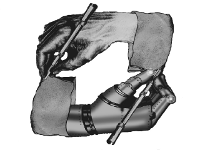
\includegraphics[width=35pt]{Figures/lacam}}

\footnotesize \let\small\footnotesize





{
  \setbeamertemplate{headline}{}
  \setbeamertemplate{footline}{}
  \begin{frame}
    \titlepage
  \end{frame}
}

\begin{frame}[fragile]
  \frametitle{Meta-rules I}
  As we have seen with searching, designing the rule set for an expert system equals to determine the
  possible transitions in the space of the WM states.\par
  In more complex context one may want to \textbf{create}, \textbf{edit} and \textbf{delete}
  rules \emph{at runtime}.\par
  CLIPS provides a primitive for deleting a rule, \textsf{undefrule}
  and one for creating them\footnote{With it it is possible to
    evaluate one \textsf{def} construct. It is similar to
    \textsf{eval}, while the latter is able to evaluate expressions
    legal in the REPL. Please refer to CLIPS Basic
    Programming Guide.}, \textsf{build}.
  \begin{clips-code}
    CLIPS> (build "(defrule foo (a) => (assert (b)))")
    TRUE
    CLIPS> (rules)
    foo
  \end{clips-code}

  However editing them at runtime is not possible in general. If a
  rule represents a graph search node transition function, one cannot
  specify a dynamic salience to represent the evaluated value for an
  heuristic considering the two states at runtime. In the same way as
  one cannot specify a dynamic and mutable LHS, since it won't compile
  in a valid part of the RETE, or as one cannot specify an uncertainty
  factor or define a partial match for the LHS.
\end{frame}

\begin{frame}
  \frametitle{Meta-rules II}
  To freely manipulate such transitions, that is to be able to govern a
  more complex strategy, one could adopt a different
  conceptualization: represent \emph{them as facts}. \par
  In a fashion we are representing our specificy control \textbf{\emph{rules as
      facts}} and leaving CLIPS rules, which can be called \textbf{meta-rules},
  to define a \emph{more general control strategy}.\par

  For instance, in a diagnostic system, if we have pieces of knowledge
  like this one:\par\bigskip
  \emph{\textbf{If} the patient has symptom A and symptom B \textbf{then} he can possibly have
  disease C.}\par\bigskip
  In our system we will encode them as some templated facts
  representing the LHS and RHS, then our rules could be something like:\par\bigskip
  \emph{\textbf{If} there is a symptom that can be asked that can lead
    to a disease we could diagnose, \textbf{then} ask about that
    symptom}\par\bigskip

  We will show how to write meta-rules for modeling a backtracking
  strategy or to implement a decision tree searching strategy.
\end{frame}

\section{Decision Trees}
{\setbeamertemplate{headline}{}
  \begin{frame}
    \sectionpage
  \end{frame}
}

\begin{frame}
  \frametitle{Tree representation I}
  
  Following the animal classification example\footnote{See
    Giarratano's \& Riley's book, chapter 12 and the provided code.},
  suppose that we possess this pieces of knowledge:\par\bigskip
  \emph{\textbf{If} the animal is not warm-blooded \textbf{then} it is a snake.}\par
  \emph{\textbf{If} the animal is warm-blooded and does not purr, \textbf{then} it is a dog.}\par
  \emph{\textbf{If} the animal is warm-blooded and does purr, \textbf{then} it is a cat.}\par\bigskip

  We will use decision trees as simple classifiers, expecting their
  inner nodes to be representing a choice to be answered (questions to
  the users); while leaves are the classification decision
  output (the animal race).\par\bigskip

  Instead of writing three CLIPS rules we will represent them with
  facts as a decision tree specifying its nodes and branches.\par
  A decision tree encodes a set of rules by compactly representing the
  patterns that appear in their LHSs.
  
\end{frame}

\begin{frame}
  \frametitle{Tree representation II: example}
  \begin{center}
    \includegraphics[width=0.7\textwidth]{Figures/dectree-1}
  \end{center}
  Each rule is represented as a path going from the root node to a
  possible leaf node.\par
  Note that we need to start from a root. What about rules without
  any pattern in common?\par\bigskip
  
  It is also possible to have decision nodes with more outgoing
  branches, i.e. representing multiple choices.
\end{frame}

\begin{frame}[fragile]
  \frametitle{Tree representation III}
  Nodes can be encoded as unordered facts with slots specifying the
  type (decision or answer) and branch type (yes-node no-node)
  and the eventual question or answer\footnote{This representation may
  be redundant, can you simplify it?}:
  \begin{clips-code}[numbers=none]
    (deftemplate node 
        (slot name) (slot type)
        (slot question) (slot yes-node)
        (slot no-node) (slot answer))
  \end{clips-code}

  The first node shall be the one named \textsf{root}.\par
  Branches are expressed by saving the yes and no child node names.\par\bigskip
  
  Additionally, a fact \textsf{current-node} may be used to keep track
  of the node we are currently exploring (by saving its name).\par
      
\end{frame}

\begin{frame}[fragile]
  \frametitle{Knowledge Base}
  In this representation, the KB will contain such nodes for our tree:
  \begin{clips-code}
    (node (name root) (type decision)  (question "Is the animal warm-blooded?") 
          (yes-node node1) (no-node node2) (answer nil))
    (node (name node1) (type decision) (question "Does the animal purr?") 
          (yes-node node3) (no-node node4) (answer nil))
    (node (name node2) (type answer) (question nil)
          (yes-node nil) (no-node nil) (answer snake))
    (node (name node3) (type answer) (question nil)
          (yes-node nil) (no-node nil) (answer cat))
    (node (name node4) (type answer) (question nil)
          (yes-node nil) (no-node nil) (answer dog))
        \end{clips-code}
        
  If we put it into a file, "ANIMAL.DAT", this would be the starting rule:
  \begin{clips-code}[numbers=none]
    (defrule initialize
        (not (node (name root)))
        =>
        (load-facts "ANIMAL.DAT") (assert (current-node root)))
  \end{clips-code}
\end{frame}

\begin{frame}[fragile]
  \frametitle{Visiting the tree I}
  Starting from the root the search advances by properly setting the
  \textsf{current-node} fact. In the case it is a decision node:
  \begin{clips-code}[numbers=none]
    (defrule ask-decision-node-question
        ?node <- (current-node ?name) (node (name ?name) (type decision)
        (question ?question))
        (not (answer ?))
        =>
        (printout t ?question " (yes or no) ")
        (assert (answer (read))))
  \end{clips-code}

  To move onto the yes or no branches, we could simply use two rules:
  \begin{clips-code}[numbers=none]
    (defrule proceed-to-yes-branch
        ?node <- (current-node ?name)
        (node (name ?name) (type decision) (yes-node ?yes-branch))
        ?answer <- (answer yes)
        =>
        (retract ?node ?answer)
        (assert (current-node ?yes-branch)))
  \end{clips-code}    
\end{frame}

\begin{frame}[fragile]
  \frametitle{Visiting the tree II}
  Whether we reach a leaf, the user can be asked if the answer is correct
  \begin{clips-code}[numbers=none]
    (defrule ask-if-answer-node-is-correct
        ?node <- (current-node ?name)
        (node (name ?name) (type answer) (answer ?value))
        (not (answer ?))
        =>
        (printout t "I guess it is a " ?value crlf)
        (printout t "Am I correct? (yes or no) ")
        (assert (answer (read)))) ;; we need to check the answer now
  \end{clips-code}

  Supposing the answer was correct, one can restart the whole process
  by resetting the \textsf{current-node} to the root:
  \begin{clips-code}[numbers=none]
    (defrule one-more-time
        ?phase <- (ask-try-again) ;; we can assert it at the end
        ?answer <- (answer yes)
        =>
        (retract ?phase ?answer)
        (assert (current-node root)))
  \end{clips-code}
      
\end{frame}


\begin{frame}[fragile]
  \frametitle{Growing the tree I}
  Supposing the answer is incorrect, we could ask the user for the
  correct animal race and try to extend the tree. This corresponds to
  modify one rule in our KB.
  \begin{clips-code}[numbers=none]
    (defrule answer-node-guess-is-incorrect
        ?node <- (current-node ?name)
        (node (name ?name) (type answer))
        ?answer <- (answer no)
        =>
        (assert (replace-answer-node ?name))
        (retract ?answer ?node))
  \end{clips-code}
  The function \textsf{replace-answer-node} has to substitute the old
  leaf with a subtree rooted in a decision node standing for a user
  supplied question, leading to a new yes branch (the correct answer)
  and a no branch (the old leaf).
      
\end{frame}

\begin{frame}[fragile]
  \frametitle{Growing the tree II}
  
  \begin{clips-code}
    CLIPS> (reset)
    CLIPS> (run)
    Is the animal warm-blooded? (yes or no) yes
    Does the animal purr? (yes or no) no
    I guess it is a dog
    Am I correct? (yes or no) no
    What is the animal? bird
    What question when answered yes will distinguish 
    a bird from a dog? Does the animal fly?
    Now I can guess bird
    Try again? (yes or no) yes
    Is the animal warm-blooded? (yes or no) yes
    Does the animal purr? (yes or no) no
    Does the animal fly? (yes or no) yes
    I guess it is a bird
    Am I correct? (yes or no) yes
    Try again? (yes or no) no
    CLIPS> 
  \end{clips-code}
  
\end{frame}

\begin{frame}
  \frametitle{Growing the tree III}
  \begin{center}
    \includegraphics[width=0.7\textwidth]{Figures/dectree-2}
  \end{center}
\end{frame}

\begin{frame}
  \frametitle{Decision trees: exercises}
Make the original code more general and totally independent from the
animal classification domain. Changing the KB containing the rules as
the decision tree is easy.\par
For instance, think about a simple decision tree to classify movies by
genre.\par\bigskip

Implement the rules presented in a simple diagnostic classifier as a
decision tree. Note how the choice of a decision node position can
change the tree structure but not the classification.\par
Can you implement a procedure (in Java for example) to
random build the tree?\par\bigskip

Extend the code to represent multiple choices decision
nodes.\par\bigskip

\end{frame}

\section{Backward chaining}
{\setbeamertemplate{headline}{}
  \begin{frame}
    \sectionpage
  \end{frame}
}

\begin{frame}
  \frametitle{A simple goal driven search}

  To implement a very simple backward chaining strategy, we will
  assume these simplifications\footnote{These examples and code are taken from
    Giarratano's and Riley's book, chapter 12.4.}:
  \begin{itemize}
  \item facts and patterns are single valued attributes (without unknown values)
  \item LHSs are conjunctions of such patterns
  \item to match a pattern we check for the equality of its value
  \item goals (and RHS) are composed by  single patterns
  \item if a goal cannot be derived by rules, it is asked to the user
  \end{itemize}\bigskip
  
  Since CLIPS inference engine implements forward chaining, a backward
  chaining system in CLIPS would need a non banal representation for
  rules and facts.\par
  The simplest thing is to use facts to represent and manipulate our
  KB rules, and defining meta rules for solving a goal by backward chaining.
\end{frame}

\begin{frame}[fragile]
  \frametitle{Backward chaining: representation}

  The module \textsf{BC} will contains our representations.\par
  Rules are unordered facts with multislots for the LHS and RHS part.
  \begin{clips-code}[numbers=none]
    (deftemplate BC::rule
        (multislot if) (multislot then))
  \end{clips-code}
  Matching is done by extracting from their lists the patterns, which are in
  the form of \textsf{attribute \textbf{is} value}. If more than one
  pattern is present in a LHS, then they are separated by the keyword
  \textbf{\textsf{and}}.\par
  This is an example for a rule as a fact from the animal domain:
  \begin{clips-code}[numbers=none]
    (rule (if warm-blooded is yes and does-purr is yes)
          (then animal is cat))
  \end{clips-code}

  In the same module we can define templates for facts keeping track
  of the facts as attributes involved in matching and the current goal:
 \begin{clips-code}[numbers=none]
    (deftemplate BC::attribute 
        (slot name) (slot value))
    (deftemplate BC::goal (slot attribute))
  \end{clips-code}
\end{frame}

\begin{frame}[fragile]
  \frametitle{Wine suggester I}
  Suppose we are modeling the knowledge for a wine suggester that
  provides the best wine color to be associated with a dish, in the
  form of these rules:\par\bigskip

  \emph{\textbf{If} the main course is red meat, \textbf{then} the best color is red}\par
  \emph{\textbf{If} the main course is fish \textbf{then} the best color is white}\par
  \emph{\textbf{If} the main course is poultry and it is turkey, \textbf{then} the best color
  is red}\par
  \emph{\textbf{If} the main course is poultry but it is not turkey, \textbf{then} the best
  color is white}\par\bigskip

According to our conceptualization we would have:
\begin{clips-code}[numbers=none]
  (deffacts MAIN::wine-rules
      (rule (if main-course is red-meat) (then best-color is red))
      (rule (if main-course is fish) (then best-color is white))
      (rule (if main-course is poultry and meal-is-turkey is yes)
            (then best-color is red))
      (rule (if main-course is poultry and meal-is-turkey is no)
            (then best-color is white)))

  (deffacts MAIN::initial-goal (goal (attribute best-color)))
\end{clips-code}
\end{frame}



% \begin{frame}[fragile]
%   \frametitle{Backward chaining: representing rules II}
%   \begin{clips-code}[numbers=none]
%     (defrule BC::attempt-rule
%         (goal (attribute ?g-name))
%         (rule (if ?a-name $?)
%         (then ?g-name $?))
%         (not (attribute (name ?a-name)))
%         (not (goal (attribute ?a-name)))
%         =>
%         (assert (goal (attribute ?a-name))))
%   \end{clips-code}
% \end{frame}

\begin{frame}
  \frametitle{Backward chaining: strategy I}
  The main strategy will revolve around trying to solve goals. We
  start with an input goal.\par\bigskip
  This is a sketch of the input procedure:

  \begin{enumerate}[I.]
  \item If a goal refers to a known asserted attribute, then the attribute
    value is returned.
  \item Otherwise, we have to \textsf{attempt} to solve each rule whose RHS contains
    our current goal. For each rule, we try to solve recursively each
    pattern in the LHS, that is we set the current goal to them and
    repeat these steps again. If the value returned is not the one we
    searched for, we remove the rule from the WM, else we remove the
    attribute from the LHS and proceed.
  \item If we were not able to satisfy the goal, we ask the user for
    the value, update the goal and return the value.
  \end{enumerate}\bigskip

  At each time, in the WM, we have the rules that we still can search
  for, the one that are unmatchable are removed. In the same way we
  remove the patterns in a LHS of a rule if they already matched some fact.
  
\end{frame}

\begin{frame}[fragile]
  \frametitle{Backward chaining: strategy II}
  Supposing our WM contains the initial asserted rules for the wine
  suggester, if we happen to know that the main disch is
  \textsf{poultry} we can remove two rules since they are not
  applicable, ending up with just:
  \begin{clips-code}[numbers=none]
    (rule (if main-course is poultry and meal-is-turkey is yes)
          (then best-color is red))
    (rule (if main-course is poultry and meal-is-turkey is no)
          (then best-color is white)))
  \end{clips-code}
  in the WM. Moreover, when we are testing for the remaining attributes
  in these rules LHSs, we can rewrite them as:
  \begin{clips-code}[numbers=none]
    (rule (if meal-is-turkey is yes)
          (then best-color is red))
    (rule (if meal-is-turkey is no)
          (then best-color is white)))
  \end{clips-code}
  Note that in this way we are forgetting the initial formulation for
  our rules. This may be crucial if we wanted to implement an
  hypothesis testing approach.      
\end{frame}

\begin{frame}[fragile]
  \frametitle{Backward chaining: strategy III}
  While attempting a rule, if we match the RHS, we have to set a new
  goal for the first attribute in the LHS:
  \begin{clips-code}[numbers=none]
    (defrule BC::attempt-rule
        (goal (attribute ?g-name))
        (rule (if ?a-name $?) (then ?g-name $?))
        (not (attribute (name ?a-name)))
        (not (goal (attribute ?a-name)))
        =>
        (assert (goal (attribute ?a-name))))
  \end{clips-code}

  If no rule and attribute can satisfy a goal, let's ask the user,
  then assert it as a fact:    
  \begin{clips-code}[numbers=none]
    (defrule BC::ask-attribute-value
        ?goal <- (goal (attribute ?g-name))
        (not (attribute (name ?g-name)))
        (not (rule (then ?g-name $?)))
        =>
        (retract ?goal)
        (printout t "What is the value of " ?g-name "? ")
        (assert (attribute (name ?g-name)  (value (read)))))
  \end{clips-code}
\end{frame}


\begin{frame}[fragile]
  \frametitle{Backward chaining: strategy IV}
  If a rule in the WM has a single pattern LHS and is satisfied,
  remove it and assert the matching fact:
  \begin{clips-code}[numbers=none]
    (defrule BC::rule-satisfied
        (declare (salience 100))
        (goal (attribute ?g-name))
        (attribute (name ?a-name) (value ?a-value))
        ?rule <- (rule (if ?a-name is ?a-value) 
                       (then ?g-name is ?g-value))
        =>
        (retract ?rule)
        (assert (attribute (name ?g-name) (value ?g-value))))
  \end{clips-code}
  If we have a matching fact for our goal, remove the goal from the WM:    
  \begin{clips-code}[numbers=none]
    (defrule BC::goal-satisfied
        (declare (salience 100))
        ?goal <- (goal (attribute ?g-name))
        (attribute (name ?g-name))
        =>
        (retract ?goal))


  \end{clips-code}
\end{frame}

\begin{frame}[fragile]
  \frametitle{Backward chaining: strategy V}
  If the rule is not applicable, just retract ii from the WM:
  \begin{clips-code}[numbers=none]
    (defrule BC::remove-rule-no-match
        (declare (salience 100))
        (goal (attribute ?g-name))
        (attribute (name ?a-name) (value ?a-value))
        ?rule <- (rule (if ?a-name is ~?a-value) 
                       (then ?g-name is ?g-value))
        =>
        (retract ?rule))

    
  \end{clips-code}
  If one\footnote{In this case always the first is checked, can you
    make match checking more flexible?} of its LHS pattern, match, just remove it (and update the rule):    
  \begin{clips-code}[numbers=none]
    (defrule BC::modify-rule-match
        (declare (salience 100))
        (goal (attribute ?g-name))
        (attribute (name ?a-name) (value ?a-value))
        ?rule <- (rule (if ?a-name is ?a-value and $?rest-if) 
                       (then ?g-name is ?g-value))
        =>
        (retract ?rule)
        (modify ?rule (if $?rest-if)))
  \end{clips-code}
\end{frame}

\begin{frame}[fragile]
  \frametitle{Wine suggester II}
  Here is a log with the the \textsf{watch facts} and \textsf{watch
    rules} commands, showing what is happening in the WM:
  \begin{clips-code}[basicstyle=\tiny]
    CLIPS> (reset)
    <== f-0     (initial-fact)
    <== f-7     (attribute (name main-course) (value poultry))
    <== f-8     (rule (if meal-is-turkey is no) (then best-color is white))
    <== f-11    (attribute (name meal-is-turkey) (value yes))
    <== f-12    (attribute (name best-color) (value red))
    ==> f-0     (initial-fact)
    ==> f-1     (rule (if main-course is red-meat) (then best-color is red))
    ==> f-2     (rule (if main-course is fish) (then best-color is white))
    ==> f-3     (rule (if main-course is poultry and meal-is-turkey is yes) (then best-color is red))
    ==> f-4     (rule (if main-course is poultry and meal-is-turkey is no) (then best-color is white))
    ==> f-5     (goal (attribute best-color))
    CLIPS> (run)
    FIRE    1 start-BC: f-0
    FIRE    2 attempt-rule: f-5,f-4,,
    ==> f-6     (goal (attribute main-course))
    FIRE    3 ask-attribute-value: f-6,,
    <== f-6     (goal (attribute main-course))
  \end{clips-code}
\end{frame}

\begin{frame}[fragile]
  \frametitle{Wine suggester III}
  \begin{clips-code}[basicstyle=\tiny,firstnumber=19]
    What is the value of main-course? poultry
    ==> f-7     (attribute (name main-course) (value poultry))
    FIRE    4 remove-rule-no-match: f-5,f-7,f-2
    <== f-2     (rule (if main-course is fish) (then best-color is white))
    FIRE    5 remove-rule-no-match: f-5,f-7,f-1
    <== f-1     (rule (if main-course is red-meat) (then best-color is red))
    FIRE    6 modify-rule-match: f-5,f-7,f-4
    <== f-4     (rule (if main-course is poultry and meal-is-turkey is no) (then best-color is white))
    ==> f-8     (rule (if meal-is-turkey is no) (then best-color is white))
    FIRE    7 modify-rule-match: f-5,f-7,f-3
    <== f-3     (rule (if main-course is poultry and meal-is-turkey is yes) (then best-color is red))
    ==> f-9     (rule (if meal-is-turkey is yes) (then best-color is red))
    FIRE    8 attempt-rule: f-5,f-9,,
    ==> f-10    (goal (attribute meal-is-turkey))
    FIRE    9 ask-attribute-value: f-10,,
    <== f-10    (goal (attribute meal-is-turkey))
  \end{clips-code}
\end{frame}

\begin{frame}[fragile]
  \frametitle{Wine suggester IV}
  \begin{clips-code}[firstnumber=35]
    What is the value of meal-is-turkey? yes
    ==> f-11    (attribute (name meal-is-turkey) (value yes))
    FIRE   10 rule-satisfied: f-5,f-11,f-9
    <== f-9     (rule (if meal-is-turkey is yes) (then best-color is red))
    ==> f-12    (attribute (name best-color) (value red))
    FIRE   11 goal-satisfied: f-5,f-12
    <== f-5     (goal (attribute best-color))
    CLIPS> (facts *)
    f-0     (initial-fact)
    f-7     (attribute (name main-course) (value poultry))
    f-8     (rule (if meal-is-turkey is no) (then best-color is white))
    f-11    (attribute (name meal-is-turkey) (value yes))
    f-12    (attribute (name best-color) (value red))
    For a total of 5 facts.
  \end{clips-code}
\end{frame}

\begin{frame}
  \frametitle{Backward chaining: exercises}
  
\end{frame}


% \section{Uncertainty}
% {\setbeamertemplate{headline}{}
%   \begin{frame}
%     \sectionpage
%   \end{frame}
% }


\end{document}


%%% Local Variables:
%%% mode: latex
%%% TeX-engine: xetex
%%% TeX-master: t
%%% End:
